\begin{frame}
	\frametitle{Table of contents}
	\tableofcontents
\end{frame}

\section{View from above}

\subsection{Domain of use}
\begin{frame}
	\frametitle{Application domain and working principle}
	
	\begin{itemize}
		\item Industrial environment.\\
		\item An energy meter sends data regarding the electric consumption of a machinery through the internet.\\
		\item Data are received, analysed and collected by the cloud application.
	\end{itemize}
	
	\bigskip
	\begin{figure}[h]
		\centering
		
\includegraphics[width=0.5\textwidth]{./img/general_domain.png}
	\end{figure}
\end{frame}


\subsection{General structure}
\begin{frame}
	\frametitle{General structure of the system}
	
	\begin{itemize}
		\item 5 microservices.
		\item Every microservice carry on a specific task.
		\item Only one entry point.
	\end{itemize}
	
	\begin{figure}[h]
		\centering
		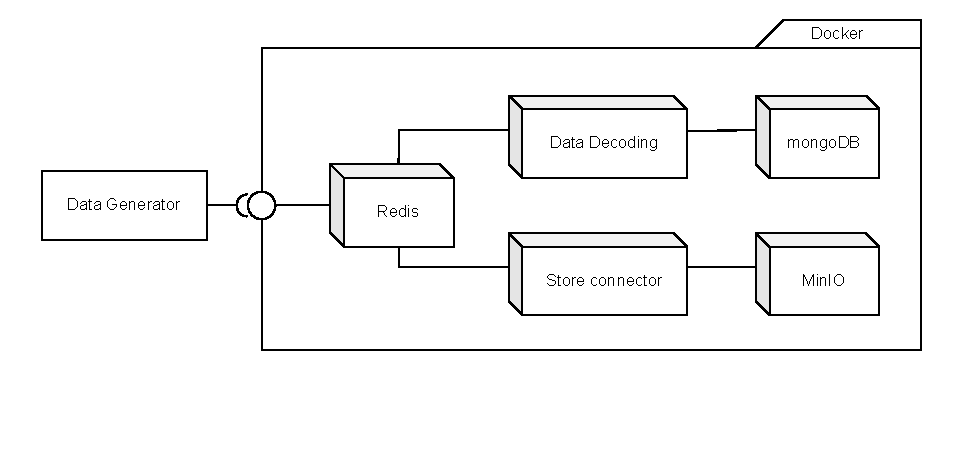
\includegraphics[width=0.8\textwidth]{./drawings/general_scheme.pdf}
	\end{figure}
\end{frame}


\section{Detailed view}

\subsection{Data Generator}
\begin{frame}
	\frametitle{Data Generator}
	
	\begin{itemize}
		\item It simulates data produced by each power meter.
		\item It publish data on a specific MQTT topic.\\
			E.g. Data from \texttt{machine1} of \texttt{customer1} are published on \texttt{data/customer1/machine1}
	\end{itemize}
	
	\bigskip
	\begin{figure}[h]
		\centering
		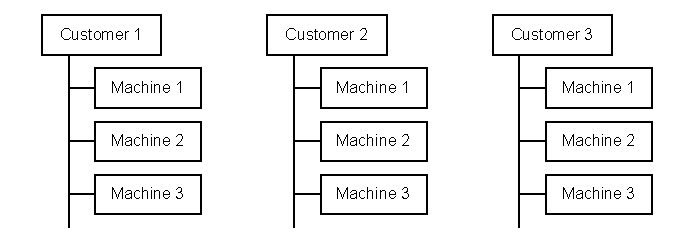
\includegraphics[width=0.6\textwidth]{./drawings/MachinesHierarchy.pdf}
	\end{figure}
\end{frame}


\subsection{Mosquitto}
\begin{frame}
	\frametitle{Mosquitto}
	
	\begin{itemize}
		\item MQTT broker.
		\item It receives data from all the meters and forward them to two microservices.
		\item It is the entry point of the entire system.
	\end{itemize}
	
	\begin{figure}[h]
		\centering
		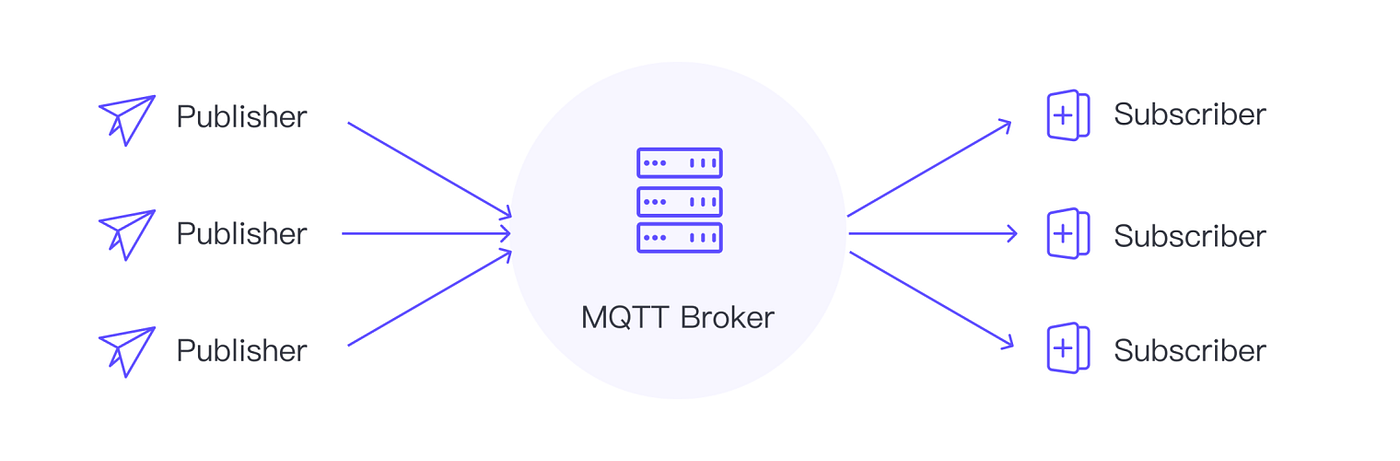
\includegraphics[width=0.7\textwidth]{./img/mqttBroker.png}
	\end{figure}
\end{frame}


\subsection{Data decoding}
\begin{frame}[containsverbatim]
	\frametitle{Data decoding}
	
	\begin{itemize}
		\item It subscribes to Mosquitto topic \verb|data/#|.
		\item It receives a hexadecimal string that is split to obtain data, hour and numeric value of the measure.\\
		E.g. \verb|'2024-09-07T19:53:19.561339'| $\rightarrow$ \verb|'1268b41553b7'|\\
		Numeric value \verb|68 DEC| $\rightarrow$ \verb|44 HEX|.\\
		Then the two strings are concatenated: \verb|'1268b41553b744'|.
		\item It prepares a JSON document and writes it into the database.
	\end{itemize}
	
	\begin{figure}[h]
		\centering
		\begin{minted}[tabsize=2, fontsize=\small]{json}
			{
				"customer": "customer1",
				"machine": "machine1",
				"date": "2024-07-18T18:05:05Z",
				"EE": 32
			}
		\end{minted}
		\caption{Example of document}
	\end{figure}
	
\end{frame}


\subsection{MongoDB Database}
\begin{frame}
	\frametitle{MongoDB Database}
	
	\begin{itemize}
		\item It stores all measurements.
		\item It provides all data if a user wants to download or visualize them.
	\end{itemize}
	
	\begin{figure}[h]
		\centering
		
\includegraphics[width=0.5\textwidth]{./img/MongoDB-Logo.png}
	\end{figure}
\end{frame}


\subsection{Store connector}
\begin{frame}[containsverbatim]
	\frametitle{Store connector}
	
	\begin{itemize}
		\item It subscribes to Mosquitto topic \verb|data/#|.
		\item It encapsulates raw data (hexadecimal strings) into text files.
		\item A unique filename is set to every file, given following this scheme
			\mintinline{python}|f"{self.machine_name}_{current_time}_{unique_id}"|,
			where \mintinline{python}|unique_id = uuid.uuid4()|.
		\item Files are sent for permanent storage.
	\end{itemize}
	
\end{frame}

\subsection{MinIO Object Store}
\begin{frame}
	\frametitle{MinIO Object Store}
	
	\begin{itemize}
		\item It is an object store platform, organized in buckets and fully compatible with Amazon S3.
		\item It takes care of the permanent storage of raw data.
		\item One bucket for each customer.
	\end{itemize}
	
	\begin{figure}[h]
		\centering
		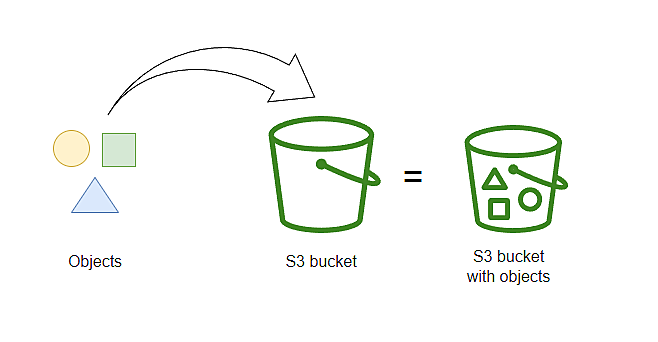
\includegraphics[width=0.5\textwidth]{./img/buckets.png}
	\end{figure}
\end{frame}





